% Created by tikzDevice version 0.7.0 on 2014-08-02 12:34:58
% !TEX encoding = UTF-8 Unicode
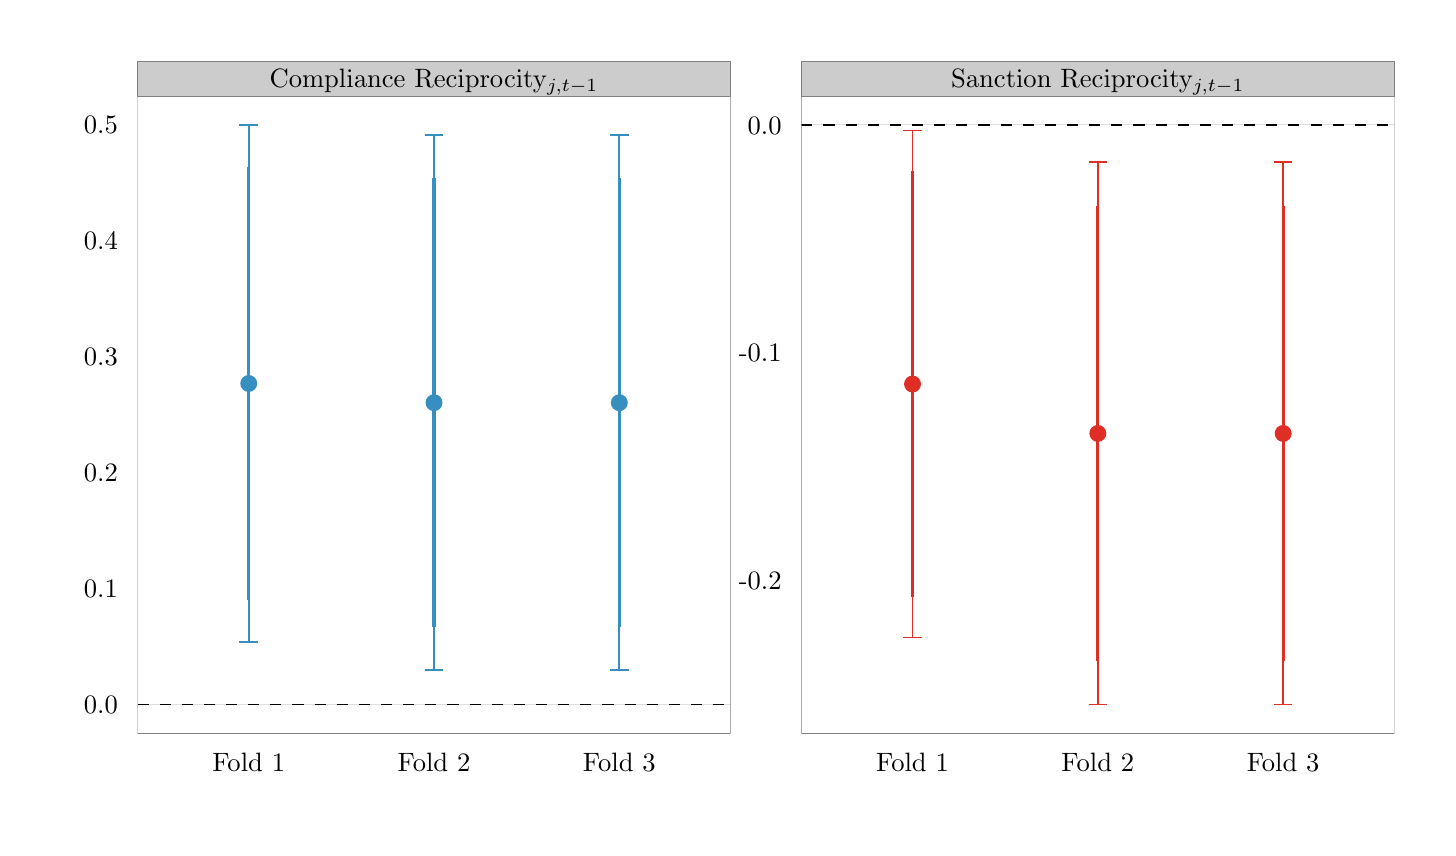
\begin{tikzpicture}[x=1pt,y=1pt]
\definecolor[named]{fillColor}{rgb}{1.00,1.00,1.00}
\path[use as bounding box,fill=fillColor,fill opacity=0.00] (0,0) rectangle (505.89,289.08);
\begin{scope}
\path[clip] (  0.00,  0.00) rectangle (505.89,289.08);
\definecolor[named]{drawColor}{rgb}{1.00,1.00,1.00}
\definecolor[named]{fillColor}{rgb}{1.00,1.00,1.00}

\path[draw=drawColor,line width= 0.6pt,line join=round,line cap=round,fill=fillColor] (  0.00,  0.00) rectangle (505.89,289.08);
\end{scope}
\begin{scope}
\path[clip] ( 39.69, 34.03) rectangle (253.97,264.40);
\definecolor[named]{fillColor}{rgb}{1.00,1.00,1.00}

\path[fill=fillColor] ( 39.69, 34.03) rectangle (253.97,264.40);
\definecolor[named]{drawColor}{rgb}{0.21,0.56,0.75}
\definecolor[named]{fillColor}{rgb}{0.21,0.56,0.75}

\path[draw=drawColor,draw opacity=0.30,line width= 0.3pt,line join=round,fill=fillColor,fill opacity=0.30] ( 79.87, 67.10) -- ( 79.87,253.93);

\path[draw=drawColor,draw opacity=0.30,line width= 0.3pt,line join=round,fill=fillColor,fill opacity=0.30] (146.83, 56.88) -- (146.83,250.25);

\path[draw=drawColor,draw opacity=0.30,line width= 0.3pt,line join=round,fill=fillColor,fill opacity=0.30] (213.79, 56.88) -- (213.79,250.25);
\definecolor[named]{drawColor}{rgb}{0.21,0.56,0.75}
\definecolor[named]{fillColor}{rgb}{0.21,0.56,0.75}

\path[draw=drawColor,line width= 1.1pt,line join=round,fill=fillColor] ( 79.87, 82.12) -- ( 79.87,238.91);

\path[draw=drawColor,line width= 1.1pt,line join=round,fill=fillColor] (146.83, 72.42) -- (146.83,234.71);

\path[draw=drawColor,line width= 1.1pt,line join=round,fill=fillColor] (213.79, 72.42) -- (213.79,234.71);
\definecolor[named]{drawColor}{rgb}{0.00,0.00,0.00}
\definecolor[named]{fillColor}{rgb}{0.00,0.00,0.00}

\path[draw=drawColor,line width= 0.6pt,dash pattern=on 4pt off 4pt ,line join=round,fill=fillColor] ( 39.69, 44.51) -- (253.97, 44.51);
\definecolor[named]{drawColor}{rgb}{0.21,0.56,0.75}
\definecolor[named]{fillColor}{rgb}{0.21,0.56,0.75}

\path[draw=drawColor,line width= 0.4pt,line join=round,line cap=round,fill=fillColor] ( 79.87,160.51) circle (  2.85);

\path[draw=drawColor,line width= 0.4pt,line join=round,line cap=round,fill=fillColor] (146.83,153.56) circle (  2.85);

\path[draw=drawColor,line width= 0.4pt,line join=round,line cap=round,fill=fillColor] (213.79,153.56) circle (  2.85);

\path[draw=drawColor,line width= 0.6pt,line join=round] ( 76.52,253.93) --
	( 83.21,253.93);

\path[draw=drawColor,line width= 0.6pt,line join=round] ( 79.87,253.93) --
	( 79.87, 67.10);

\path[draw=drawColor,line width= 0.6pt,line join=round] ( 76.52, 67.10) --
	( 83.21, 67.10);

\path[draw=drawColor,line width= 0.6pt,line join=round] (143.48,250.25) --
	(150.18,250.25);

\path[draw=drawColor,line width= 0.6pt,line join=round] (146.83,250.25) --
	(146.83, 56.88);

\path[draw=drawColor,line width= 0.6pt,line join=round] (143.48, 56.88) --
	(150.18, 56.88);

\path[draw=drawColor,line width= 0.6pt,line join=round] (210.45,250.25) --
	(217.14,250.25);

\path[draw=drawColor,line width= 0.6pt,line join=round] (213.79,250.25) --
	(213.79, 56.88);

\path[draw=drawColor,line width= 0.6pt,line join=round] (210.45, 56.88) --
	(217.14, 56.88);
\definecolor[named]{drawColor}{rgb}{0.50,0.50,0.50}

\path[draw=drawColor,line width= 0.6pt,line join=round,line cap=round] ( 39.69, 34.03) rectangle (253.97,264.40);
\end{scope}
\begin{scope}
\path[clip] (279.56, 34.03) rectangle (493.85,264.40);
\definecolor[named]{fillColor}{rgb}{1.00,1.00,1.00}

\path[fill=fillColor] (279.56, 34.03) rectangle (493.85,264.40);
\definecolor[named]{drawColor}{rgb}{0.87,0.18,0.15}
\definecolor[named]{fillColor}{rgb}{0.87,0.18,0.15}

\path[draw=drawColor,draw opacity=0.30,line width= 0.3pt,line join=round,fill=fillColor,fill opacity=0.30] (319.74, 68.71) -- (319.74,251.88);

\path[draw=drawColor,draw opacity=0.30,line width= 0.3pt,line join=round,fill=fillColor,fill opacity=0.30] (386.70, 44.51) -- (386.70,240.42);

\path[draw=drawColor,draw opacity=0.30,line width= 0.3pt,line join=round,fill=fillColor,fill opacity=0.30] (453.67, 44.51) -- (453.67,240.42);
\definecolor[named]{drawColor}{rgb}{0.87,0.18,0.15}
\definecolor[named]{fillColor}{rgb}{0.87,0.18,0.15}

\path[draw=drawColor,line width= 1.1pt,line join=round,fill=fillColor] (319.74, 83.44) -- (319.74,237.16);

\path[draw=drawColor,line width= 1.1pt,line join=round,fill=fillColor] (386.70, 60.25) -- (386.70,224.67);

\path[draw=drawColor,line width= 1.1pt,line join=round,fill=fillColor] (453.67, 60.25) -- (453.67,224.67);
\definecolor[named]{drawColor}{rgb}{0.00,0.00,0.00}
\definecolor[named]{fillColor}{rgb}{0.00,0.00,0.00}

\path[draw=drawColor,line width= 0.6pt,dash pattern=on 4pt off 4pt ,line join=round,fill=fillColor] (279.56,253.93) -- (493.85,253.93);
\definecolor[named]{drawColor}{rgb}{0.87,0.18,0.15}
\definecolor[named]{fillColor}{rgb}{0.87,0.18,0.15}

\path[draw=drawColor,line width= 0.4pt,line join=round,line cap=round,fill=fillColor] (319.74,160.30) circle (  2.85);

\path[draw=drawColor,line width= 0.4pt,line join=round,line cap=round,fill=fillColor] (386.70,142.46) circle (  2.85);

\path[draw=drawColor,line width= 0.4pt,line join=round,line cap=round,fill=fillColor] (453.67,142.46) circle (  2.85);

\path[draw=drawColor,line width= 0.6pt,line join=round] (316.39,251.88) --
	(323.09,251.88);

\path[draw=drawColor,line width= 0.6pt,line join=round] (319.74,251.88) --
	(319.74, 68.71);

\path[draw=drawColor,line width= 0.6pt,line join=round] (316.39, 68.71) --
	(323.09, 68.71);

\path[draw=drawColor,line width= 0.6pt,line join=round] (383.35,240.42) --
	(390.05,240.42);

\path[draw=drawColor,line width= 0.6pt,line join=round] (386.70,240.42) --
	(386.70, 44.51);

\path[draw=drawColor,line width= 0.6pt,line join=round] (383.35, 44.51) --
	(390.05, 44.51);

\path[draw=drawColor,line width= 0.6pt,line join=round] (450.32,240.42) --
	(457.01,240.42);

\path[draw=drawColor,line width= 0.6pt,line join=round] (453.67,240.42) --
	(453.67, 44.51);

\path[draw=drawColor,line width= 0.6pt,line join=round] (450.32, 44.51) --
	(457.01, 44.51);
\definecolor[named]{drawColor}{rgb}{0.50,0.50,0.50}

\path[draw=drawColor,line width= 0.6pt,line join=round,line cap=round] (279.56, 34.03) rectangle (493.85,264.40);
\end{scope}
\begin{scope}
\path[clip] (  0.00,  0.00) rectangle (505.89,289.08);
\definecolor[named]{drawColor}{rgb}{0.50,0.50,0.50}
\definecolor[named]{fillColor}{rgb}{0.80,0.80,0.80}

\path[draw=drawColor,line width= 0.2pt,line join=round,line cap=round,fill=fillColor] ( 39.69,264.40) rectangle (253.97,277.04);
\definecolor[named]{drawColor}{rgb}{0.00,0.00,0.00}

\node[text=drawColor,anchor=base,inner sep=0pt, outer sep=0pt, scale=  0.96] at (146.83,267.41) {Compliance Reciprocity$_{j,t-1}$};
\end{scope}
\begin{scope}
\path[clip] (  0.00,  0.00) rectangle (505.89,289.08);
\definecolor[named]{drawColor}{rgb}{0.50,0.50,0.50}
\definecolor[named]{fillColor}{rgb}{0.80,0.80,0.80}

\path[draw=drawColor,line width= 0.2pt,line join=round,line cap=round,fill=fillColor] (279.56,264.40) rectangle (493.85,277.04);
\definecolor[named]{drawColor}{rgb}{0.00,0.00,0.00}

\node[text=drawColor,anchor=base,inner sep=0pt, outer sep=0pt, scale=  0.96] at (386.70,267.41) {Sanction Reciprocity$_{j,t-1}$};
\end{scope}
\begin{scope}
\path[clip] (  0.00,  0.00) rectangle (505.89,289.08);
\definecolor[named]{drawColor}{rgb}{0.00,0.00,0.00}

\node[text=drawColor,anchor=base east,inner sep=0pt, outer sep=0pt, scale=  0.96] at ( 32.57, 41.20) {0.0};

\node[text=drawColor,anchor=base east,inner sep=0pt, outer sep=0pt, scale=  0.96] at ( 32.57, 83.15) {0.1};

\node[text=drawColor,anchor=base east,inner sep=0pt, outer sep=0pt, scale=  0.96] at ( 32.57,125.09) {0.2};

\node[text=drawColor,anchor=base east,inner sep=0pt, outer sep=0pt, scale=  0.96] at ( 32.57,167.04) {0.3};

\node[text=drawColor,anchor=base east,inner sep=0pt, outer sep=0pt, scale=  0.96] at ( 32.57,208.98) {0.4};

\node[text=drawColor,anchor=base east,inner sep=0pt, outer sep=0pt, scale=  0.96] at ( 32.57,250.93) {0.5};
\end{scope}
\begin{scope}
\path[clip] (  0.00,  0.00) rectangle (505.89,289.08);
\definecolor[named]{drawColor}{rgb}{0.00,0.00,0.00}

\node[text=drawColor,anchor=base east,inner sep=0pt, outer sep=0pt, scale=  0.96] at (272.45, 86.05) {-0.2};

\node[text=drawColor,anchor=base east,inner sep=0pt, outer sep=0pt, scale=  0.96] at (272.45,168.34) {-0.1};

\node[text=drawColor,anchor=base east,inner sep=0pt, outer sep=0pt, scale=  0.96] at (272.45,250.62) {0.0};
\end{scope}
\begin{scope}
\path[clip] (  0.00,  0.00) rectangle (505.89,289.08);
\definecolor[named]{drawColor}{rgb}{0.00,0.00,0.00}

\node[text=drawColor,anchor=base,inner sep=0pt, outer sep=0pt, scale=  0.96] at ( 79.87, 20.31) {Fold 1};

\node[text=drawColor,anchor=base,inner sep=0pt, outer sep=0pt, scale=  0.96] at (146.83, 20.31) {Fold 2};

\node[text=drawColor,anchor=base,inner sep=0pt, outer sep=0pt, scale=  0.96] at (213.79, 20.31) {Fold 3};
\end{scope}
\begin{scope}
\path[clip] (  0.00,  0.00) rectangle (505.89,289.08);
\definecolor[named]{drawColor}{rgb}{0.00,0.00,0.00}

\node[text=drawColor,anchor=base,inner sep=0pt, outer sep=0pt, scale=  0.96] at (319.74, 20.31) {Fold 1};

\node[text=drawColor,anchor=base,inner sep=0pt, outer sep=0pt, scale=  0.96] at (386.70, 20.31) {Fold 2};

\node[text=drawColor,anchor=base,inner sep=0pt, outer sep=0pt, scale=  0.96] at (453.67, 20.31) {Fold 3};
\end{scope}
\end{tikzpicture}
